\documentclass{beamer}

\mode<presentation> {

    \usetheme{Madrid}
    \usecolortheme{beaver}
}

\usepackage{graphicx}

%--------------------------------------------------
% Title Page
%--------------------------------------------------

\title[git]{A short introduction to git}
\author{John Ladan}
\institute[Waterloo]{University of Waterloo\\john@ladan.ca}
\date{\today}

\begin{document}

\begin{frame}
    \titlepage
\end{frame}

\begin{frame}
    \frametitle{Overview}
    \tableofcontents
\end{frame}

%--------------------------------------------------
% Presentation slides
%--------------------------------------------------

\section{What is git?}

\begin{frame}
    \frametitle{According to git-scm.com}
    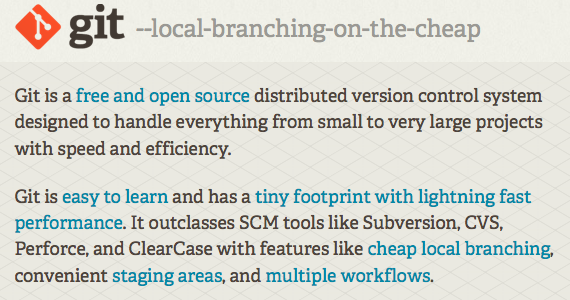
\includegraphics{figures/git-homepage}
\end{frame}

\begin{frame}
    \frametitle{According to wikipedia.org}
    Git (/ɡɪt/) is a distributed revision control system with an emphasis on speed, data integrity, and support for distributed, non-linear workflows. Git was initially designed and developed by Linus Torvalds for Linux kernel development in 2005, and has since become the most widely adopted version control system for software development.

    As with most other distributed revision control systems, and unlike most client–server systems, every Git working directory is a full-fledged repository with complete history and full version-tracking capabilities, independent of network access or a central server. Like the Linux kernel, Git is free software distributed under the terms of the GNU General Public License version 2.
\end{frame}

\begin{frame}
    \frametitle{Features}
    \begin{itemize}
        \item Fast
        \item Nonlinear development (via rapid branching, and DAG based structure)
        \item Distributed -- each copy of the repo is complete by itself
            \begin{itemize}
                \item each copy of the repo is itself a repo
                \item changes can be pushed/pulled to any other instance
                \item do not need network access
            \end{itemize}
        \item Ubiquitous
    \end{itemize}
\end{frame}

% Probably something about github here

\section{Cloning a Repo}

% git clone <repository location>
% at this point, it's basically just like downloading a tarball, because it's file-based
% an advantage of git: don't need to compile tarball, tags, partial pull
% may run into submodules

\section{Making Changes}

% Always branch first, because
% - it's a good habit
% - the last good state is labelled (often as master)
% - can go back to another branch even if you're in the middle of something
% - can update master w/o a merge conflicting with current changes
% - branches are cheap!
%
% Next, Make your changes
% - edit things however you like
% - it's best to use `git rm` or `git mv` for file manipulation
%
% Stage files:
% - git add <file>
%
% Check Status:
% - git status
%
% Commit:
% - git add <file>; git commit ... or git commit -a
% - commits should be small, and non-breaking (if possible)
% - best to keep one commit to one feature/bugfix
% - recommend not using the `-m` option, because of bash history

\section{Starting Your Own}

% Typical case:
% - start coding
% - git init
% - create a remote repo
% - add the remote as origin
% - push --set-upstream
%
% With Foresight:
% - create a repo (on github)
% - clone that repo to your machine
% - start coding

\section{Version Control}

% What's this HEAD thing, and all those numbers? (commit hash)
% Tagging
% master branch
% undoing changes that haven't been committed
% going back a bit further (HEAD~1)

\section{In Practice}

% - `git status` will tell you most of what you need (it suggests commands)
% - create an alias for glog
% - search for how to do things on google
% - forking and pull requests
% - github
% - git stash & git stash pop (made changes but forgot to branch)
% - for your own project, it should be more linear
% - delete your old branches (after they're merged back in)
% - `git commit --amend` to fix that last commit
